
% !TEX root = ./../main.tex

\section{Case Study: Bellevue - a Verified Graphical Editor}
\label{sec:case-study}

This chapter presents the design and implementation of the \emph{Bellevue} graphical editor.
It illustrates how to build a complex application with \ac{COP}, and the bugs that one may encounter due to inconsistent interactions between layers.


%%
\subsection{Case Study Design}
\label{sec:design}

Bellevue is a graphical editor that was developed as a case study to demonstrate the use of Refinement Types in the verification of consistency between layer interactions in \ac{COP} programs.
The main features of Bellevue are:

\begin{enumerate}[label=(\arabic*)]
  \item Drawing basic pre-defined geometric shapes such as rectangles and circles.
  \item Free hand drawing with a brush by clicking and dragging the mouse over the screen
  \item An eraser
  \item Color fill an arbitrary delimited area using a simple flood-fill algorithm
  \item Selection of colors, brush sizes, eraser radius and other settings
\end{enumerate}

The overall structure of the application follows the \emph{Elm} architecture with three core components~\cite{ElmLang2025}:
\begin{enumerate*}[label=(\arabic*)]
  \item the \textbf{Model}, which represents the current state of the application,
  \item the \textbf{View}, which specifies how the \textbf{Model} is rendered into HTML and
  \item the \textbf{Update} function, which specifies how the \textbf{Model} should be updated upon receiving a \textbf{Message}.
\end{enumerate*}

The execution flow of the application is determined by the \textbf{Messages} that are being exchanged between the browser and the application. A \textbf{Message} describes an event that occurred within the application;
for example, the action of clicking a button sends a \textbf{Message} with data that describes such action and information associated with the button.
The \textbf{Update} function then has to determine, for each \textbf{Message} type, how the state should change (if at all), and what additional actions should be performed.
These actions are modeled as \textbf{Commands}, and they describe the side effects that need to be performed by the application.
Actions like logging messages, making HTTP requests or drawing into an HTML Canvas, are some examples of \textbf{Commands}

This architectural style was mainly chosen for its simplicity. Since the Elm architecture is a purely functional approach for implementing web applications, it is easier to integrate with the
\emph{Stainless} framework, which is a verifier mainly intended for functional programs.

\begin{figure}[h]
  \centering
  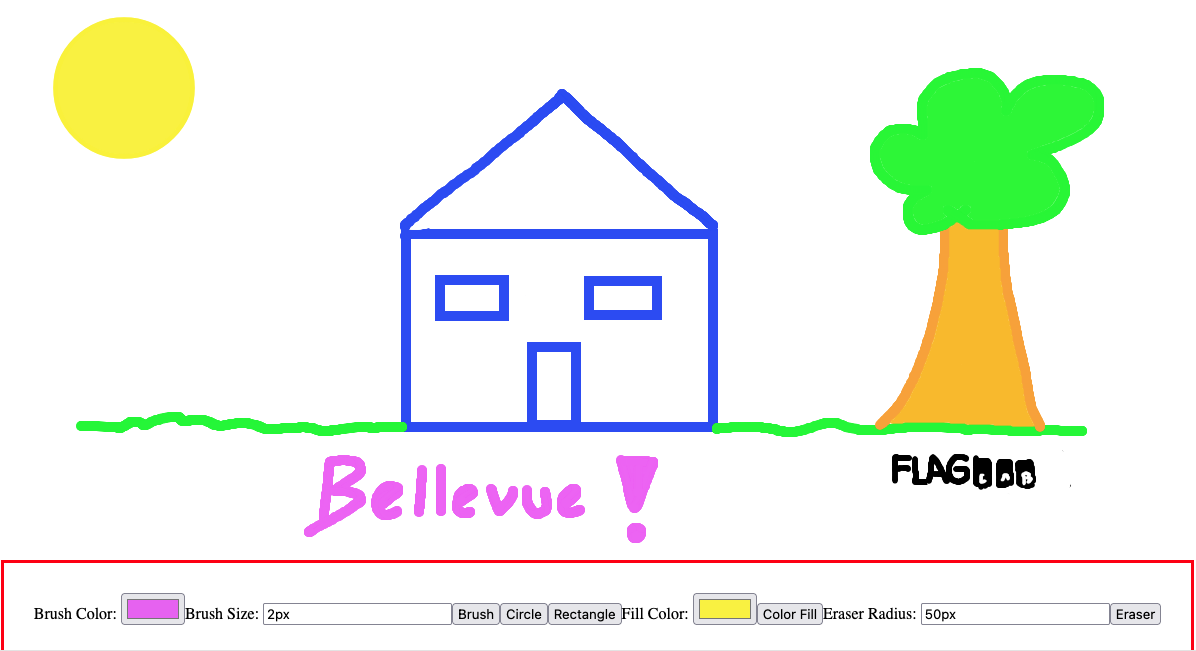
\includegraphics[width=14cm]{figures/BellevueExample}
  \caption{Bellevue}
  \label{fig:bellevue}
\end{figure}

\fref{fig:bellevue} shows a view of the Bellevue editor with its drawing tools and features.
The full implementation of the application can be found in the following repository: \url{https://github.com/slemus9/bellevue}

\section{Implementation}

The \textbf{Model} of the application is represented by the \lstinline|DrawingModel| class in \fref{lst:bellevue-model}. It contains data about
the current selected tool, the styling configuration chosen by the user and the state of the mouse interaction, among other things.

\begin{scala}[label=lst:bellevue-model, caption=Bellevue Model]
final case class DrawingModel(
    selectedTool: Tool,
    brushConfig: StyleConfig,
    colorFillConfig: ColorFillConfig,
    eraserConfig: EraserConfig,
    mouseDragging: Option[MouseDragging],
    receivedMessage: Msg
)
\end{scala}

The \lstinline|Tool| type in \fref{lst:bellevue-tool} represents a drawing tool that can be selected by the user, and it is modelled as a simple enumeration.

\begin{scala}[label=lst:bellevue-tool, caption=Bellevue drawing tools]
enum Tool:
  case Brush, ColorFill, Circle, Eraser, Rectangle
\end{scala}

The mouse interaction is represented by the \lstinline|MouseDragging| class in \fref{lst:bellevue-mouse-dragging}.
All drawing actions are performed through mouse dragging: the user clicks on any point in the canvas, then drags the mouse across it, and finally releases the mouse.
A \lstinline|MouseDragging| instance holds the starting position at which the mouse was clicked, and the latest position that was recorded while the mouse was being dragged.

\begin{scala}[label=lst:bellevue-mouse-dragging, caption=Bellevue mouse dragging modelling]
final case class MouseDragging(
    startPosition: Point,
    latestPosition: Point
)
\end{scala}

Finally, \lstinline|Msg| is a Sum Type of all types of \textbf{Messages} that can be exchanged in the application:

\begin{scala}[label=lst:bellevue-msg]
type Msg = ControlMsg | MouseMsg | ToolboxMsg

enum ControlMsg:
  case HtmlElementLoaded(id: String)
  case MapToCanvas(point: Point, toMouseMsg: Point => MouseMsg)
  case NoAction
  case ResizeCanvas

enum MouseMsg:
  case MouseDown(point: Point)
  case MouseMove(point: Point)
  case MouseUp(point: Point)

enum ToolboxMsg:
  case PickBrushSize(size: Pixels)
  case PickColor(color: RGB)
  case PickEraserRadius(radius: Pixels)
  case PickFillColor(color: RGB)
  case PickTool(tool: Tool)
  case SetCanvasImage(image: Image)
\end{scala}

The logic of the application is defined within the \textbf{Update} function. The \emph{Tyrian}~\cite{Indigoengine2025} front-end framework was used for this case study to implement Bellevue. It provides an abstraction to develop
web applications based on the Elm architecture, and the \textbf{Update} function signature is:

\begin{scala}[label=lst:bellevue-update-signature]
def update(model: DrawingModel): Msg => (DrawingModel, Cmd)
\end{scala}

Given a current \lstinline|model| and a \textbf{Message} of type \lstinline|Msg|, the \lstinline|update| function returns a new
\lstinline|DrawingModel| together with a \textbf{Command} (side effect) of type \lstinline|Cmd|, that may or may not produce a new \textbf{Message}.
Instead of explicitly dispatching all types of messages in a single pattern matching block, the \textbf{Update} function is implemented as the composition of several \textbf{Predicated Functions},
each of them describing a particular drawing interaction, that is implicitly activated as specified by their \lstinline|isActive| predicate.

For instance, \fref{lst:bellevue-brush-action} shows the definition of \lstinline|BrushAction|, a \textbf{Predicated Function} that draws into the canvas whenever the user wants to perform
a free-hand drawing using a "brush".

\begin{scala}[label=lst:bellevue-brush-action, caption=Free hand brush drawing action]
object BrushAction extends PredicatedFunction[DrawingModel, Cmd]:

  override def isActive(state: DrawingModel): Boolean =
    state.selectedTool == Tool.Brush &&
      state.receivedMessage.isInstanceOf[MouseMsg] &&
      state.mouseDragging.isDefined

  override val run: Behavior[DrawingModel, Cmd] = prevAction => model =>
    (model.receivedMessage, model.mouseDragging) match
      case (MouseMsg.MouseMove(to), Some(dragging)) =>
        val from = dragging.latestPosition
        val drawSegment = canvas.drawLineSegment(from, to)
        (model, prevAction |+| drawSegment)

      case (MouseMsg.MouseUp(to), Some(dragging)) =>
        val from = dragging.latestPosition
        val drawSegment = canvas.drawLineSegment(from, to)
        (model, prevAction |+| drawSegment)
\end{scala}

Only when the selected tool is a \lstinline|Brush| and the user is performing a mouse drag, will the
\lstinline|BrushAction| draw a small line segment between the latest position recorded and the position to which the mouse was dragged at.
Note that the \lstinline|drawSegment| side effect is being concatenated to the previous action's side effect using the |+| operator; this means
that the action of drawing a line segment will be executed alongside with whatever action was previously active.

For the drawing to be consistent, the model needs to be updated so that the \lstinline|mouseDragging| object accurately reflects the user's actions.
A separate Predicated Function can be defined just for this purpose, as shown in \fref{lst:bellevue-mouse-drag-update-action}.

\begin{scala}[label=lst:bellevue-mouse-drag-update-action, caption=Action to update the mouse dragging state]
object MouseDragUpdateAction extends PredicatedFunction[DrawingModel, Cmd]:

  override def isActive(state: DrawingModel): Boolean =
    state.receivedMessage.isInstanceOf[MouseMsg]

  override val run: Behavior[DrawingModel, Cmd] = prevAction => model =>
    model.receivedMessage match
      case MouseMsg.MouseDown(from) => (model.clickMouse(from), prevAction)
      case MouseMsg.MouseMove(to)   => (model.moveMouse(to), prevAction)
      case MouseMsg.MouseUp(_)      => (model.releaseMouse, prevAction)
\end{scala}

The \lstinline|MouseDragUpdateAction| updates the \lstinline|mouseDragging| state whenever a \lstinline|MouseMsg| was received.
Note that this action does not perform any side effects on its own, as it only returns the previous active action's side effect. The only thing it does,
is update the model in accordance to the received mouse positions. If the user clicked the mouse (\lstinline|MouseDown|), it will create a new
\lstinline|MouseDragging| instance using the mouse position as the \lstinline|startPosition|. If the user is moving the mouse around (\lstinline|MouseMove|), then it will
set the \lstinline|latestPosition| of the \lstinline|mouseDragging| state to the current mouse position. Otherwise, if the user releases the mouse (\lstinline|MouseUp|), it will
set the \lstinline|mouseDragging| state to \lstinline|None|, signaling that the mouse drag interaction ended.

\begin{scala}[label=lst:bellevue-mouse-drag-update-action-aux, caption=Complementary functions to update the mouse dragging state]
  def clickMouse(startPosition: Point) =
    copy(mouseDragging = Some(MouseDragging.init(startPosition)))

  def moveMouse(to: Point) =
    this.focus(_.mouseDragging.some.latestPosition).replace(to)

  def releaseMouse =
    copy(mouseDragging = None)
\end{scala}

Since most drawing actions are mouse dragging interactions, abstracting this behavior into a separate \lstinline|MouseDragUpdateAction| function enables better reusability.
Actions like drawing rectangles or erasing are similar to the \lstinline|BrushAction| function, and they also rely on a proper model update of the \lstinline|mouseDragging| state.
\fref{lst:bellevue-common-draw-actions-predicates} shows the activation predicates for some common drawing actions:

\begin{scala}[label=lst:bellevue-common-draw-actions-predicates, caption=Common drawing actions predicates]
// Draws rectangles
object RectangleAction extends PredicatedFunction[DrawingModel, Cmd]:

  override def isActive(state: DrawingModel): Boolean =
    state.selectedTool == Tool.Rectangle &&
      state.receivedMessage.isInstanceOf[MouseMsg]

// Draws circles
object CircleAction extends PredicatedFunction[DrawingModel, Cmd]:

  override def isActive(state: DrawingModel): Boolean =
    state.selectedTool == Tool.Circle &&
      state.receivedMessage.isInstanceOf[MouseMsg]

// Erases drawings by painting circles of the same color as the background
object EraserCanvasAction extends PredicatedFunction[DrawingModel, Cmd]:

  override def isActive(state: DrawingModel): Boolean =
    state.selectedTool == Tool.Eraser &&
      state.mouseDragging.isDefined &&
      state.receivedMessage.isInstanceOf[MouseMsg]
\end{scala}

Each function defines how to manipulate the canvas independently, but they all should receive a consistent \lstinline|mouseDragging| state.
To make sure this is the case, the functions can be composed with the \lstinline|MouseDragUpdateAction| as shown in the following code snippet:

\begin{scala}[label=lst:bellevue-draw-actions-composition, caption=Drawing actions composition]
val DrawAction: PredicatedFunction[DrawingModel, Cmd] =
  PredicatedFunction.sequence(
    PredicatedFunction.oneOf(
      BrushAction,
      CircleAction,
      EraserAction,
      RectangleAction
    ),
    MouseDragUpdateAction
  )
\end{scala}

The implementation of the remaining Bellevue features follow the same structure; canvas and state manipulation are separated into different Predicated Functions,
and they are later composed in the proper order. Finally, there is a single \lstinline|BellevueAction| function that comprises all functionality, and it is then used to define the body of the
\textbf{Update} function

\begin{scala}[label=lst:bellevue-update-function-def, caption=Bellevue Update function definition]
val BellevueAction: PredicatedFunction[DrawingModel, Cmd] =
  PredicatedFunction.oneOf(DrawAction, ...)

def update(model: DrawingModel): Msg => (DrawingModel, Cmd) =
  msg => BellevueAction.runWith(model.withMessage(msg), Cmd.None)
\end{scala}


%%
\subsection{Verification with Refinement Types}
\label{sec:verification}

A total of 15 Predicated Functions are defined to specify the \textbf{Update} function.
All of them should be composed in the right order, and there are implicit dependencies between the activation conditions of some of the functions.
While developing the case study without Refinement Types, most of the bugs introduced in the application were due to inconsistencies in the interaction between the functions.
In \fref{sec:preliminaries.cop}, we defined a layer interaction as the dependency that is formed between two layers, due to the fact that the state manipulation and Behavior of one layer, may affect the activation and Behavior of another one.
In terms of \lstinline|PredicatedFunctions|, these interactions are materialized by applying our composition functions (\lstinline|sequence| and \lstinline|orElse|), and they can result in an inconsistent behavior depending on the definition of the activation predicate and \lstinline|Behavior| of each function.
We have already seen some examples of inconsistent interactions in \fref{sec:context-scala.refined-predicated-functions}, where \lstinline|PredicatedFunctions| can be activated or deactivated due to the \lstinline|Behavior| of a previous active function.
In this section we identify two classes of errors that arise from inconsistent interactions, and we illustrate how these issues can be detected at compile-time using our approach.

The first class of identified errors, is the rendering of incorrect drawings due to incorrectly-ordered compositions.
For instance, if the \lstinline|MouseDragUpdateAction| is placed as the first function of the composition in \fref{lst:bellevue-draw-actions-composition}, some of the drawings will be inconsistent with respect to the user actions.
This is because, if a \lstinline|MouseUp| message is received, the \lstinline|releaseMouse| state modification sets the \lstinline|mouseDragging| value to \lstinline|None|, even when the other functions still need it to perform some operations in the canvas.
For example, circles would not be drawn at all, since the \lstinline|MouseUp| event marks the point where the user wants to display the final shape.
To prevent this type of errors, we can rely on the \lstinline|Chainable| type from \fref{sec:context-scala.refined-predicated-functions} to verify that the activation and state manipulation of one function, does not deactivate a subsequent function in the composition.

\begin{scala}[label=lst:enforcing-dependencies, caption=Enforcing dependencies between two Predicated Functions, escapechar=~]
final class BrushAction extends PredicatedFunction[DrawingModel, Cmd]:
  override def isActive(state: DrawingModel): Boolean =
    state.selectedTool == Tool.Brush &&
      state.receivedMessage.isInstanceOf[MouseMsg] &&
      state.mouseDragging.isDefined
  ...

final class MouseDragUpdateAction extends PredicatedFunction[DrawingModel, Cmd]:
  override def isActive(state: DrawingModel): Boolean =
    state.receivedMessage.isInstanceOf[MouseMsg]
  ...

// Compiles successfully:
val validChain = new Chainable[DrawingModel, Cmd]:
  override def first = new BrushAction
  override def second = new MouseDragUpdateAction

// Stainless produces compilation error:
val invalidChain = new Chainable[DrawingModel, Cmd]:
  override def first = new MouseDragUpdateAction
  override def second = new BrushAction
\end{scala}

In \fref{lst:enforcing-dependencies}, the \lstinline|validChain| value compiles successfully because the following typing judgement is valid:

\begin{equation}
\begin{split}
isChainable &: (previous: Cmd) \\
            &\rightarrow (state: DrawingModel) \\
            &\rightarrow unit\{BrushAction.isActive(state) \\
            &\Rightarrow MouseDragUpdateAction.isActive(BrushAction.run(previous, state).first)\}
\end{split}
\end{equation}

Recall from \fref{lst:bellevue-brush-action} that \lstinline|BrushAction| returns the previous state without modifications in all of its branches,
and thus $BrushAction.run(previous, state).first = state$, reducing the type definition to:

\begin{equation}
\begin{split}
isChainable &: (previous: Cmd) \\
            &\rightarrow (state: DrawingModel) \\
            &\rightarrow unit\{BrushAction.isActive(state) \\
            &\Rightarrow MouseDragUpdateAction.isActive(state)\}
\end{split}
\end{equation}

\noindent
Where the inner implication $BrushAction.isActive(state) \Rightarrow MouseDragUpdateAction.isActive(state)$ further reduces to:

\begin{equation}
\label{eqn:brush-mouse-drag-impl}
\begin{split}
(selectedTool = Brush & \; \wedge \; receivedMessage \; : \; MouseMsg \\
  & \; \wedge \; isDefined(mouseDragging)) \\
  & \Rightarrow receivedMessage \; : \; MouseMsg
\end{split}
\end{equation}

The \ac{SMT} solver accepts the implication from Equation \ref{eqn:brush-mouse-drag-impl} as a valid formula due to the fact that, for any propositions $A$ and $B$, the formula $A \wedge B \Rightarrow B$ (and $A \wedge B \Rightarrow A$) is a tautology.
On the contrary, \lstinline|invalidChain| does not compile because an implication in the opposite direction does not hold.
These values are static checks showing that \lstinline|BrushAction| must necessarily go before \lstinline|MouseDragUpdateAction| in the composition chain,
preventing the programmer from misordering the Predicated Functions.

This approach can be repeated for all function interactions that need to be verified. Recall from \fref{lst:bellevue-draw-actions-composition}, that \lstinline|BrushAction| is not the only function that must go before \lstinline|MouseDragUpdateAction|.
The former is also accompanied by more alternative functions inside the \lstinline|oneOf| composition, and thus, the previous dependency relation must also be guaranteed
for all of these functions. In order to achieve this, the programmer can define an auxiliary property that verifies that this implication is satisfiable for a given list of Predicated Functions, as illustrated in \fref{lst:enforcing-multiple-dependencies}.

\begin{scala}[label=lst:enforcing-multiple-dependencies, caption=Enforcing dependencies between multiple Predicated Functions, escapechar=~]
def oneOfLaw(previous: Cmd, state: DrawingModel): Boolean =
  val drawActions     = List(
    new BrushAction,
    new CircleAction,
    new ColorFillAction,
    new RectangleAction
  )
  val mouseDragUpdate = new MouseDragUpdateAction

  drawActions.forall { action =>
    action.isActive(state) ==> {
      val (newState, _) = action.run(previous, state)
      mouseDragUpdate.isActive(newState)
    }
  }.holds
\end{scala}

The second class of common mistakes consists on overspecifying some of the activation predicates. For instance, one may think that it makes sense to add the \lstinline|state.mouseDragging.isDefined| condition to the \lstinline|isActive| predicate of \lstinline|RectangleAction|, just as it was done in the \lstinline|BrushAction|'s activation predicate.
However, the \lstinline|RectangleAction| also needs to display an overlaid element to highlight the place where the rectangle will be drawn in the canvas, and this is done when \lstinline|state.mouseDragging| is equal to \lstinline|None| (as soon as the new mouse dragging interaction starts). Hence, adding the new condition will make this piece of logic
to be silently ignored, as there is no static guarantee that the \lstinline|run| function definition respects the assumptions from the \lstinline|isActive| predicate:

\begin{scala}[label=lst:malformed-rectangle-action, caption=Example bug in RectangleAction, escapechar=~]
// Example of an ill-specified predicated function for drawing rectangles
object MalformedRectangleAction extends PredicatedFunction[DrawingModel, Cmd]:

  override def isActive(state: DrawingModel): Boolean =
    state.selectedTool == Tool.Rectangle &&
      state.receivedMessage.isInstanceOf[MouseMsg] &&
      state.mouseDragging.isDefined // <-- adding this condition introduces a bug


  override val run: Behavior[DrawingModel, Cmd] = prev => model =>
    (model.receivedMessage, model.mouseDragging) match
      case (MouseMsg.MouseDown(from), None) =>
        // This piece of code is unreachable ~\label{ln:malformed-rectangle-action.unreachable}~
        (model, prev |+| overlaidRectangle.show)

      case (MouseMsg.MouseMove(to), Some(dragging)) =>
        val rectangle = Rectangle(from = dragging.startPosition, to)
        (model, prev |+| overlaidRectangle.draw(rectangle))

      case (MouseMsg.MouseUp(to), Some(dragging)) =>
        val rectangle = Rectangle(from = dragging.startPosition, to)
        val draw = canvas.drawRectangle(rectangle) |+| overlaidRectangle.hide
        (model, prev |+| draw)

      case _ => (model, prev)
\end{scala}

\fref{ln:malformed-rectangle-action.unreachable} of \fref{lst:malformed-rectangle-action} states that the piece of code that makes the overlaid rectangle visible is ignored,
because the \lstinline|run| function patten matching specifies that it should be done when \lstinline|state.mouseDragging =   None|, but the Behavior of \lstinline|MalformedRectangleAction| will only be executed when \lstinline|state.mouseDragging| is defined, directly contradicting the assumptions from the \lstinline|run| function.

Most bugs that are caused by inconsistent predicates can be detected by adding the \lstinline|isActive| predicate as a pre-condition to the \lstinline|run| function.
This way, it can be guaranteed that the \lstinline|run| function respects the assumptions from the activation predicate, and Stainless will raise an error if there are inconsistencies.
In this case, we could bring the \lstinline|isActive| assumptions to the \lstinline|run| function, and then formulate a property asserting that the overlaid rectangle should always be visible when a mouse dragging interaction starts.
\fref{ln:refined-rectangle-action.property} of \fref{lst:refined-rectangle-action} shows a property asserting that for all \lstinline|prev: Cmd| and \lstinline|model: DrawingModel| values, the \lstinline|RefinedRectangleAction| should display the overlaid rectangle whenever there is a mouse-down interaction, and the \lstinline|mouseDragging| state is set to \lstinline|None|.
This will detect the unreachable code bug encountered previously, because there is no possibility that \lstinline|overlaidRectangle.isVisible| variable will be set to true, due to the additional \lstinline|state.mouseDragging.isDefined| precondition

\begin{scala}[label=lst:refined-rectangle-action, caption=Enforcing activation assumptions in the RectagleAction, escapechar=~]
final class RefinedRectangleAction extends PredicatedFunction[DrawingModel, Cmd]:

  override def isActive(state: DrawingModel): Boolean =
    state.selectedTool == Tool.Rectangle &&
      state.receivedMessage.isInstanceOf[MouseMsg] &&
      state.mouseDragging.isDefined // <-- adding this condition introduces a bug

  override def run(prev: Cmd, model: DrawingModel): Cmd =
    require(this.isActive(model)) // <-- add precondition
    ...

// This property will fail because the precondition is not met
def overlaidRectVisibleWhenMouseDragging( ~\label{ln:refined-rectangle-action.property}~
    prev: Cmd,
    model: DrawingModel
    mouseDown: MouseMsg.MouseDown
): Boolean =
  val action = new RefinedRectangleAction
  val inputModel  = model.copy(
    selectedTool = Tool.Rectangle,
    receivedMessage = Msg.Mouse(mouseDown),
    mouseDragging = None()
  )
  // The following call violates the activation precondition:
  val (_, result) = action.run(prev, inputModel)
  result.overlaidRectangle.isVisible
\end{scala}

Though these bugs may seem simple and easy to avoid, they can be hard to detect due to the high decoupling between activation and behavior.
As the application's complexity increases and new Predicated Functions are defined, the difficulty of finding these simple bugs increases, since there may be more interactions that need to be taken into account.


%%
\subsection{Discussion}
\label{sec:discussion}

Throughout the development of this case study, various challenges when creating \ac{COP} applications were evidenced,
and an alternative approach was explored to mitigate those challenges using Refinement Types.
Some of the main findings encountered while designing and implementing this approach are:

\begin{itemize}
  \item
    Refinement Types are a convenient verification tool because they are integrated with the language in which the application is being implemented, allowing the programmer to verify the actual code that is going to be executed.
    However, there were some limitations while trying to integrate with existing code and libraries for this case study. Though Stainless offers an \lstinline|@extern| annotation to do this incorporation, some Scala compiler errors were encountered during type checking.
    For instance, it was not possible to use the Tyrian framework's \lstinline|Cmd[F, A]| type inside the signature of the \lstinline|PredicatedFunction|

  \item
    Due to the difficulty of integrating with existing code, a separate notion of \textbf{Commands} had to be implemented in the Stainless \emph{Pure Scala} language subset, which then had to be translated to the Tyrian framework's \lstinline|Cmd[F, A]| type.
    This translation process introduces an additional layer of code in the application that is not verified, so further testing or verification needs to be done to cover it.
    Unfortunately, this opposes the expectation that was held at the beginning of this work, regarding a seamless code integration when using Refinement Types.

  \item
    Refinement Types were successfully used to verify some of the main interactions between Predicated Functions in this case study.
    Though the defined properties and dependency relations are specific to the needs of this particular application, it is believed that Refinement Types (and Stainless) is a sufficiently robust tool to reason about many other properties of \ac{COP} programs.

  \item
    The design choices that were made to implement \lstinline|PredicatedFunctions| and the \text{Bellevue} application facilitated the process of formal verification.
    The \lstinline|PredicatedFunction| composition naturally fits into the Elm architecture, since the signature of the \textbf{Update} function is very similar to the definition of a \lstinline|PredicatedFunction|.
    The Elm architecture, in turn, made it easier to apply Refinement Types, as we take on a Purely Functional approach of implementing the application, which is a paradigm well suited for Stainless.

  \item
    The \lstinline|Chainable| abstraction is enough to verify dependencies between two Predicated Functions, however it is not very ergonomic as the programmer has to manually construct these instances for all pair of functions that need to be verified.
    Furthermore, for composition chains longer than two functions, a transitive relation between \lstinline|Chainable|s must be established for full correctness. An attempt was made to formulate a more ergonomic \lstinline|Chainable| abstraction for multiple functions while enforcing transitivity, but unfortunately it was not completed for this case study.

  \item
    Another disadvantage of the \lstinline|Chainable| abstraction, is that is not integrated yet with the \lstinline|sequence| and \lstinline|oneOf| composition functions. So, if the programmer forgets to construct a \lstinline|Chainable| instance, these composition functions can still be used to potentially construct unsound Predicated Functions.
    A more principled approach would be to define \lstinline|andThen| and \lstinline|orElse| operations in such a way that they receive a \lstinline|Chainable| instance as an argument, which serves as an \emph{evidence} that two functions can be composed because the given dependency property holds.
    This way, it is mandatory for the programmer to verify these dependency relations before building compositions.

  \item
    More work can be done to verify more complex properties in this application regarding state transitions. For example, there is a \lstinline|ColorFill| action that contains the logic of flood-filling a closed area with a selected color.
    This Predicated Function requires the current bitmap of the canvas to be given (i.e. there is a \lstinline|.canvasImage.isDefined| condition in the activation predicate). It would be desirable to verify that the \lstinline|ColorFillAction| \emph{always} receives such bitmap when the selected tool is equal to \lstinline|Tool.ColorFill|.
    The reason why this property is harder to check with the current abstractions, is because the action that sets the bitmap is not directly chained with the \lstinline|ColorFillAction|, since they happen at two separate time instances.
    A way to tackle this would be to extend the abstractions developed in this work so that the programmer reason about state transitions, and possibly base such implementation in Temporal Logic.
\end{itemize}


\endinput

